\section{Metodología utilizada}


\subsection{Base de datos utilizada}

\vspace{5 mm}

A continuación hablaremos sobre la base de datos que hemos utilizado, los inconvenientes que hemos encontrado al usarla y como los hemos solucionado.

La base de datos que hemos usado se llama \textbf{Vietnamese Foods} y la subío un estudiante de la VNU HCMC a la web \textbf{kaggle}. Este dataset consta de 24474 imágenes divididas en 29 clases. Las imágenes no fueron previamente divididas en un set de entrenamiento y un set de test. Tampoco disponíamos de un archivo de texto con la ruta de todas las imágenes del dataset por lo que tuvimos que construirlo a mano usando la orden \textbf{find} que nos proporciona el terminal de Linux.

Una vez obtenido dicho archivo de texto con las imágenes nos fue sencillo construir los correspondientes sets de entrenamiento y test. Tuvimos que cargar todas las imágenes con sus respectivas clases en dos ndarrays, y usarlos en la función \textbf{train\_test\_split} de sklearn con un 0.2 de tamaño de test. Como las clases que usamos eran de tipo string, tuvimos que hacer uso también de la función \textbf{to\_categorical} para convertirlas en valores enteros.

Una vez intentamos cargar las imágenes en memoria nos dimos cuenta que no era posible debido al costo computacional que requería almacenar tantas imágenes en la RAM. Por este motivo redujimos el número de clases de forma aleatoria hasta llegar a \textbf{9}, que era el máximo número de clases que podíamos cargar en Google Colab sin sobrepasar sus recursos computacionales. Hemos decidido tomar esta decisión en lugar de reducir el número de imágenes de cada clase y mantener el número de clases ya que esto generaría una falta de datos a la hora de entrenar cada clase. Cabe destacar que todas las clases del dataset están equilibradas. A continuación mostraré ejemplos de las diferentes imágenes que se pueden encontrar en el dataset usado:

\vspace{5 mm}

\begin{figure}[H]
  \centering
  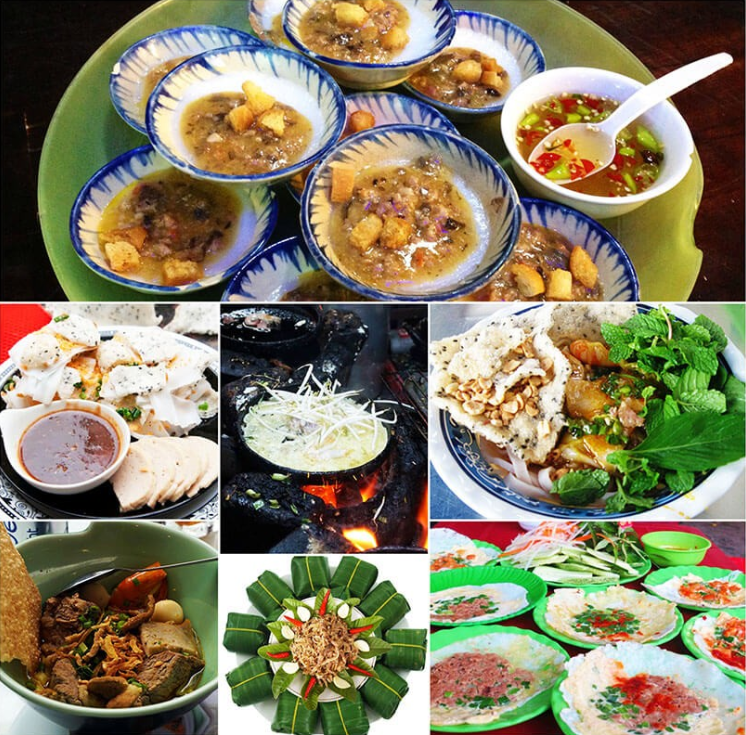
\includegraphics[width=0.5\linewidth]{Imagenes/comida-vietnamita.png}
  \caption{Imágenes del dataset Vietnamese Foods}
  \label{fig:sub-first}
\end{figure}

\newpage

\subsection{Preprocesado de los datos}

Para el preprocesado de los datos a utilizar simplemente hemos utilizado la función de preprocesado de cada red utilizada. Además de esto también hemos redimensionado las imágenes al leerlas de cara a que tengan el mismo tamaño que la entrada de las distintas redes.

También mencionar que este preprocesado se ha aplicado también al conjunto de test a la hora de predecir los valores, como vimos que es necesario tanto en teoría como en la práctica 2.


\subsection{Redes neuronales convolucionales entrenadas con ImageNet utilizadas}

\vspace{5 mm}



\subsection{Mejoras sobre las redes utilizadas}
